\section{Introduction}

The document contains requirement specification for the Le'Chuck's Morris. The document also contains constraints in our chosen COTS in addition to literature references.

\subsection{Concept}

\begin{wrapfigure}{L}{0.5\textwidth}
\vspace{-30pt}
\begin{center}
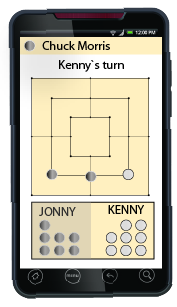
\includegraphics{concept.png}
\end{center}
\caption{Conceptual game screen}

\end{wrapfigure}


The game is based on the concept of \emph{Nine Men's Morris}, and is \newline developed by Ole Jørgen Rishoff, Stian Sørebø, Emil Andreas Mork, and Steinar Haram.
It is an abstract strategy board game for two players that emerged from the Roman Empire. Each player has nine pieces, or "men", that move among the board's twenty-four spots. The goal of the game is to leave the opposing player with fewer than three pieces or, as in checkers, no legal moves. The way to remove one of the components pieces, is to get your own pieces in a three in a row position. The functional requirements in the next section will reflect these game rules, and also cover other more specific scenarios. 



